\chapter{Programmbeschreibung}\label{ch:programmbeschreibung}


\begin{figure}
    \centering
    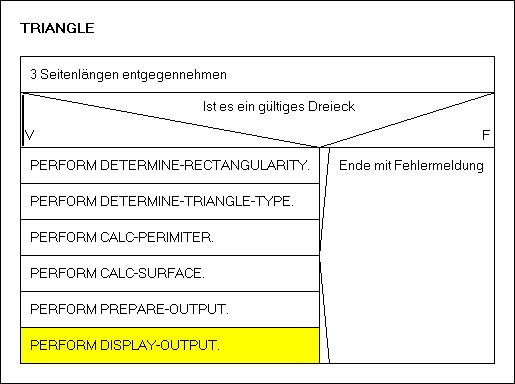
\includegraphics[width=0.5\textwidth]{images/Programmablauf.jpg}
    \caption{Programmablauf}
\end{figure}



\begin{figure}
    \centering
    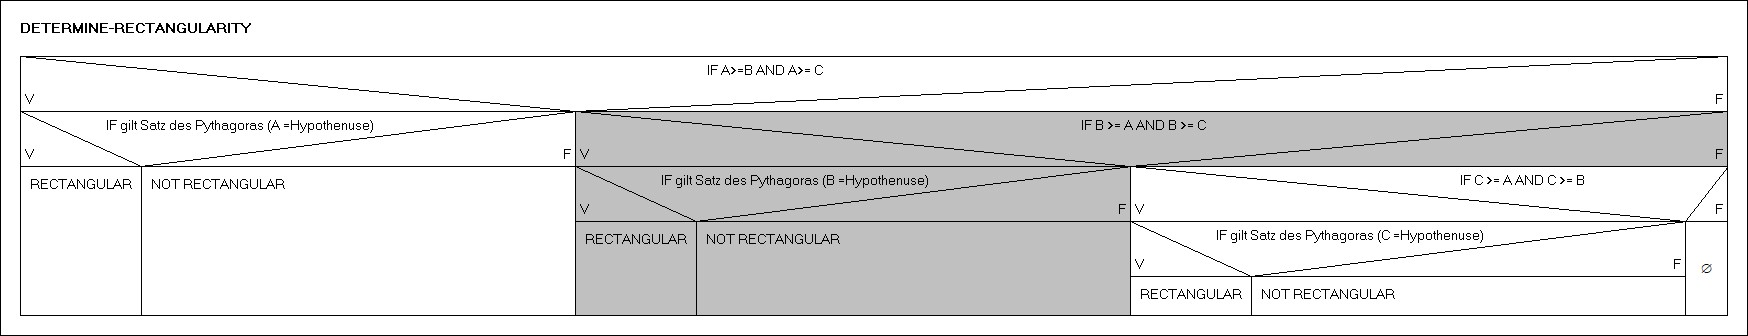
\includegraphics[width=0.5\textwidth]{images/DETERMINE RECTANGULARITY.jpg}
    \caption{Winkelart}
\end{figure}

\begin{figure}
    \centering
    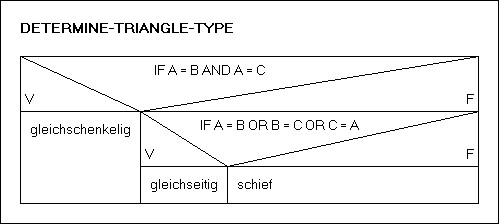
\includegraphics[width=0.5\textwidth]{images/DETERMINE-TRIANGLE-TYPE.jpg}
    \caption{Dreiecksart}
\end{figure}

\begin{figure}
    \centering
    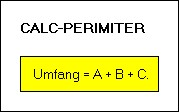
\includegraphics[width=0.5\textwidth]{images/CALC-PERIMITER.jpg}
    \caption{Umfang}
\end{figure}

\begin{figure}
    \centering
    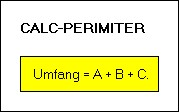
\includegraphics[width=0.5\textwidth]{images/CALC-PERIMITER.jpg}
    \caption{Oberfläche}
\end{figure}

\begin{figure}
    \centering
    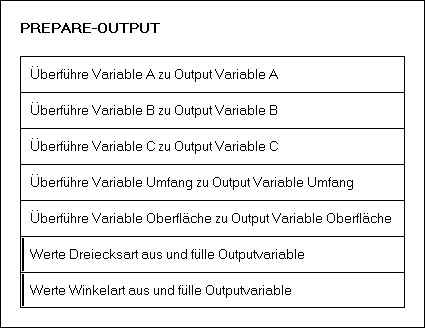
\includegraphics[width=0.5\textwidth]{images/Prepare Output.jpg}
    \caption{Ausgabevorbereitung}
\end{figure}

\begin{figure}
    \centering
    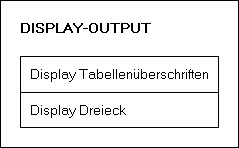
\includegraphics[width=0.5\textwidth]{images/display_output.jpg}
    \caption{Ausgabe}
\end{figure}
